\chapter{Optical Activity in Hyper-Rayleigh Scattering}\label{sec:results:HRS}

Sections of this chapter are based on the (submitted) manuscript \textit{``First observation of optical activity in hyper-Rayleigh scattering''}.
I designed the nonlinear experimental setup. H.-H. Jeong and P. Fischer fabricated the samples. HRS data were collected by myself, K. R. Rusimova, and D. C. Hooper. Linear optical data were collected by myself, K. R. Rusimova, and F. Pradaux-Caggiano. I analysed both the HRS and linear data. I produced the manuscript draft on which this chapter is based.

\bigskip \noindent
As discussed in the previous chapter, separating true chirality of nanomaterials from structural anisotropy is a major challenge. This chapter discusses an experiment designed to entirely remove anisotropic contributions to nonlinear chiroptical measurements in nanostructures: The first observation of optical activity in hyper-Rayleigh scattering (HRS). The effect is demonstrated in a 3D isotropic suspension of Ag nanohelices in water, and shows a complete sign reversal depending on handedness, as would be expected from an intrinsically-chiral origin. Moreover, the effect is significantly stronger than linear optical activity, and is well-pronounced above the multiphoton luminescence background. Because of its sensitivity, isotropic environment, and straightforward experimental geometry, HRS optical activity constitutes a fundamental experimental breakthrough in chiral photonics, for media including nano/metamaterials and chemical molecules. 


\section{Introduction}

With the invention of the laser, access to high intensity light enabled the discovery of nonlinear optical counterparts of optical activity (section~\ref{sec:background:NonlinearOptics:chirality}). However, nonlinear chiroptical techniques have not been widely adopted as routine chiroptical probes. A major drawback is that sum-frequency generation (SFG) intensities cannot distinguish between left and right-handed molecules~\cite{Valev2013b}. 
Second-harmonic processes require symmetry-breaking interfaces and, as shown in section\ref{sec:background:NonlinearOptics:chirality}, are more widely used in the chiroptical characterisation of solids than liquids. In solids however molecules can exhibit anisotropy that can easily mask the chiral response by contributing to linear dichroism, linear birefringence and circular birefringence~\cite{Kuroda2001}.
Furthermore, in solid samples, disentangling chirality from anisotropy effects is challenging, particularly for nonlinear optics~\cite{Hooper2017} (section~\ref{sec:results:OAinPlanarNanohelices}). More chiroptical processes have been reported in higher order nonlinearities, for instance, two-photon absorption circular dichroism~\cite{Tinoco1975, DeBoni2008, Toro2010} – a third order process. However, higher order nonlinearities are generally weaker, and the associated experimental techniques are complex. Therefore, nonlinear optical effects capable of distinguishing chiral forms in a liquid are highly desirable. 

This chapter discusses the observation of optical activity in hyper-Rayleigh scattering (HRS), 5 orders of magnitude more pronounced than linear OA when considering the volume of optical interaction. HRS~\cite{Clays1991b, Clays1992} occurs when incident light at a fundamental frequency is scattered at the second harmonic frequency, and is used to determine the symmetry of randomly oriented molecules in a liquid~\cite{Verbiest1994a}.
These experiments made use of sub-wavelength silver chiral nanohelices suspended in water, to form a meta-molecular liquid, and demonstrate a strong HRS signal, well distinguishable above multiphoton luminescence. Polarisation analyses of the HRS establishes that the nanohelices are isotopically arranged in the liquid. The nanohelices give rise to an HRS-CID signal that reverses for opposite chirality of the nanohelices and is much larger than the two- and three-photon luminescence CID. Moreover, the HRS and HRS-CID signals follow variations in fundamental wavelength. Crucially, in comparison to linear OA, the HRS-CID only occurs near the focal point of light, which opens up a range of applications in tiny volumes of liquids. 
In HRS-CID, incident light at a frequency $\omega$ is left- circularly polarised (LCP) or right-circularly polarised (RCP). Meta-molecules in a liquid scatter the incident light into the second-harmonic frequency $2\omega$. This hyper-Rayleigh scattered light can be detected at $\SI{90}{\degree}$ to the incident beam propagation direction. Due to the chirality of the scatterers, HRS of different intensity is produced for LCP and RCP light.


\section{Results}

\begin{figure}[htb!]	
    \centering	
    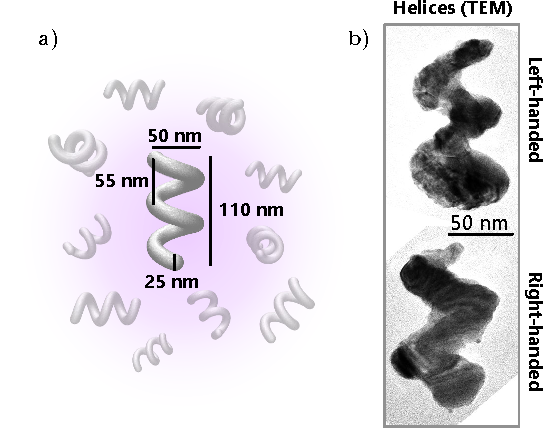
\includegraphics[scale=1]{./figures/results/HRS/sample_schematic.pdf}
    \caption{\label{fig:results:HRS:sample_schematic}
    \textbf{a)} Dimensions (center-to-centre) of the nanohelices isotropically dispersed in water. Helix height is $\SI{110}{\nano\m}$, loop diameter is $\SI{50}{\nano\m}$, loop pitch is $\SI{55}{\nano\m}$, and wire-diameter is $\SI{25}{\nano\m}$. \textbf{b)} Transmission Electron Microscopy (TEM) images of left- and right-handed helices. }	
\end{figure}

\begin{figure}[htb!]	
    \centering	
    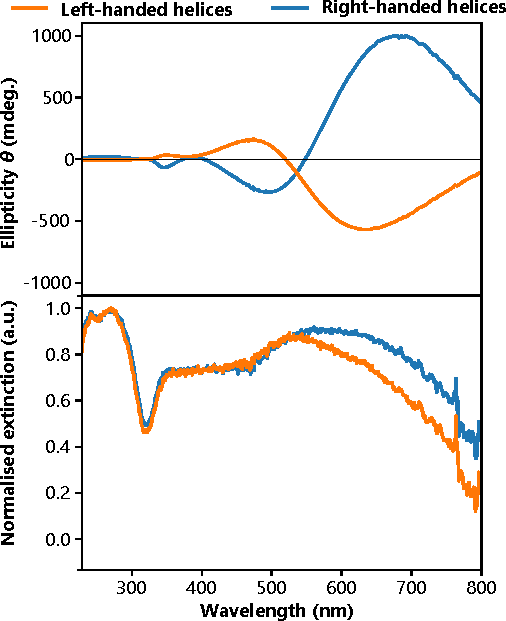
\includegraphics[scale=1]{./figures/results/HRS/linear_data.pdf}
    \caption{\label{fig:results:HRS:linear_data}
    Linear characterisation of the nanohelix solutions. \textbf{Top:} ellipticity spectra, as measured with a CD spectrometer, through a $\SI{1}{\centi\m}$ path length filled with left- and right-handed nanohelix suspensions. \textbf{Bottom:} corresponding normalised extinction spectra from the left- and right-handed nanohelix suspensions. Extinction is obtained from the transmission spectrum and describes both absorption and scattering losses.}	
\end{figure}

The nanostructures are Ag nanohelices, fabricated by H.-H. Jeong and P. Fischer using a glancing-angle shadow growth method~\cite{Gibbs2014}, and suspended in water. 
Additionally, 3-5$\%$ Ti is co-deposited with the Ag, in order to improve the structural fidelity of the nanoparticles while causing little change in their optical properties~\cite{Larsen2014b}. The Ti results in a rapidly forming oxide layer at room temperature, which quickly saturates at 3-$\SI{5}{\nano\m}$. Since Ti is more reactive with oxygen than Ag at room temperature, this becomes the dominant oxide layer. 
In principle, this layer changes the optical properties of the helices, however once the layer has rapidly formed, it grows extremely slowly (taking approximately a year to grow from $\SI{4}{\nano\m}$ to $\SI{5}{\nano\m}$~\cite[\S 7.3]{Brunette2001}). 
Therefore, the oxide layer will not change significantly over the course of the experiment. Additionally, since the layer has already formed from oxygen exposure, it protects the Ag from any further degradation while suspended in water.
For these experiments, Ag nanohelices were used over Au nanohelices (such as those examined in chapter~\ref{sec:results:OAinPlanarNanohelices}) due to exhibiting a stronger plasmon resonance at a given geometry and volume. The results presented below make use of several incident wavelengths, and thus the broader resonance of dispersed nanoparticles allows measurable signal to be obtained over a wider spectral range.

The nanohelices' dimensions, presented in figure~\ref{fig:results:HRS:sample_schematic}a, are substantially smaller than the wavelength of illumination ($\SI{720}{\nano\m}$-$\SI{780}{\nano\m}$). Since the wire radius ($\SI{12.5}{\nano\m}$) is comparable to the skin depth of Ag for $\SI{760}{\nano\m}$ light~\cite{Johnson1972}, each helix acts as a continuous helical arrangement of effective dipoles. Transmission Electron Microscopy (TEM) images of both chiral forms (enantiomorphs) are shown in figure~\ref{fig:results:HRS:sample_schematic}b. 
After fabrication on Si wafers, the wafers are cut into $\SI{1}{\centi\meter\squared}$ pieces that are each sonicated into $\SI{1.4}{\milli\litre}$ water, with $\SI{1}{\milli\mole}$ of sodium citrate stabiliser to create $\approx 20$ picomolar suspensions. These suspensions are stable over several days and can be dispensed into standard glass cuvettes for characterisation with linear and nonlinear optical techniques.  

Figure~\ref{fig:results:HRS:linear_data} shows linear ellipticity and extinction spectra (upper and lower panels respectively) for both enantiomorphs, obtained using a commercial Applied Photophysics Chirascan. A $\text{N}_2$-cooled Xe arc lamp is linearly polarised and spectrally separated in space with a pair of prisms, and a variable-width slit is used to select a wavelength with $\SI{0.1}{\nano\m}$ resolution. A photoelastic modulator (PEM) modulates the beam between LCP and RCP states, which is then directed through the sample cuvette and onto a photomultiplier tube (PMT) detector. The Chirascan then simultaneously measures total extinction and circular dichroism and constructs spectral data by scanning the wavelength.
The ellipticity $\theta$ is a measure of the CD:
\begin{equation}
    \theta (\text{deg.}) = \frac{180}{\pi} \tan\left( \frac{\sqrt{I_{RCP}} - \sqrt{I_{LCP}}}{\sqrt{I_{RCP}} + \sqrt{I_{LCP}}} \right) \approx \frac{180}{\pi} \Delta A \left( \frac{\ln 10}{4} \right)
\end{equation}
where $I_{RCP}$ and $I_{LCP}$ denote the intensity of RCP and LCP light, respectively, and $\Delta A = A_{LCP} - A_{RCP}$ is the difference in the attenuation of LCP and RCP light transmitted through the cuvette. 
The ellipticity spectra exhibit a characteristic bisignate signature that reverses with the handedness of the nanohelices. Their small asymmetry in peak maxima is due to a slight difference in concentration, attributable to experimental variation in the sonication process. Additionally, because the two chiral forms of the nanohelices are grown separately, small imperfections in the structural dimensions are also present, resulting in a slight shift in peak wavelength. The small effect of these imperfections can be seen from the extinction spectra, where the lines deviate only above $\SI{550}{\nano\m}$. The extinction is proportional to both the absorption and the scattering from the nanohelices; such scattering can also occur at the second harmonic frequency of illumination. 

\begin{figure}[htb!]	
    \centering	
    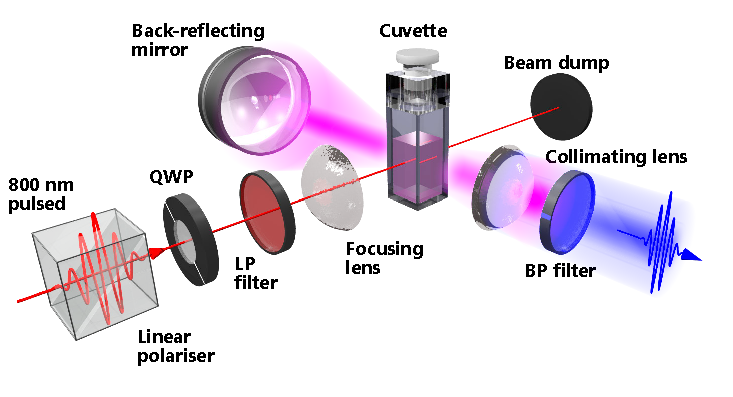
\includegraphics[scale=1]{./figures/results/HRS/experiment_schematic.pdf}
    \caption{\label{fig:results:HRS:experiment_schematic}
    Schematic diagram of the hyper-Rayleigh scattering circular dichroism experimental setup. QWP: quarter wave-plate; LP filter: long-pass filter; BP filter: band pass filter. }	
\end{figure}

Figure~\ref{fig:results:HRS:experiment_schematic} shows the experimental setup used to measure HRS-CD. 
$\SI{18.9}{\milli\watt}\pm\SI{0.1}{\milli\watt}$ of pulsed light ($\SI{139}{\kilo\watt}$ peak power, appendix~\ref{sec:appendix:hardware:maitai}) with a tunable centre wavelength, was horizontally polarised (p-polarisation), before passing through a quarter-wave plate mounted in an automatic rotation stage to give LCP or RCP light. An RG665 long pass filter removed any existing SHG from the beam, before a $\SI{100}{\milli\m}$ focal-length achromatic lens focused the incident light onto our cuvette. A $\SI{50}{\milli\m}$ focal-length collection lens positioned $\SI{50}{\milli\m}$ from the cuvette, along with a $\SI{50}{\milli\m}$ focal length curved mirror positioned $\SI{100}{\milli\m}$ from the opposite side of the cuvette, collected and collimated scattered light. A $\SI{200}{\milli\m}$ focal length lens then focused the collected light through one of several band-pass filters, onto a photomultiplier tube (PMT). The PMT output was pre-amplified and sent to an SRS SR400 Gated Photon Counter. 
By changing the band-pass filter, in $\SI{10}{\nano\m}$ increments, a spectrum of the multiphoton scattering is measured.

\begin{figure}[htb!]	
    \centering	
    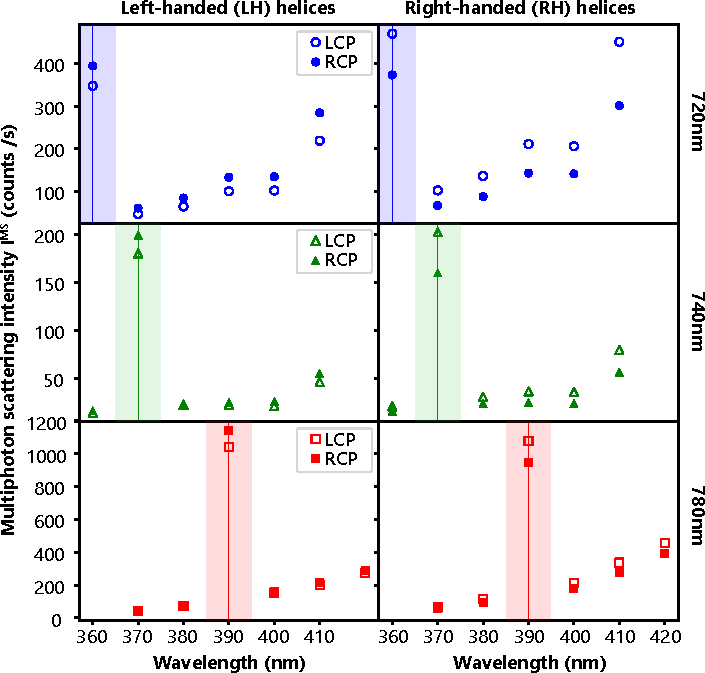
\includegraphics[scale=1]{./figures/results/HRS/hrs_data.pdf}
    \caption{\label{fig:results:HRS:hrs_data}
    Multi-photon scattering spectra for left- and right-handed helices, under LCP and RCP illumination. Results obtained for fundamental wavelengths of $\SI{720}{\nano\m}$, $\SI{740}{\nano\m}$ and $\SI{780}{\nano\m}$ are shown in blue, green, and red, respectively. Vertical coloured lines mark the HRS (second-harmonic) wavelength, demonstrating clear peaks above the multiphoton luminescence background. The HRS unambiguously follows variations of the fundamental. }	
\end{figure}

\begin{figure}[htb!]	
    \centering	
    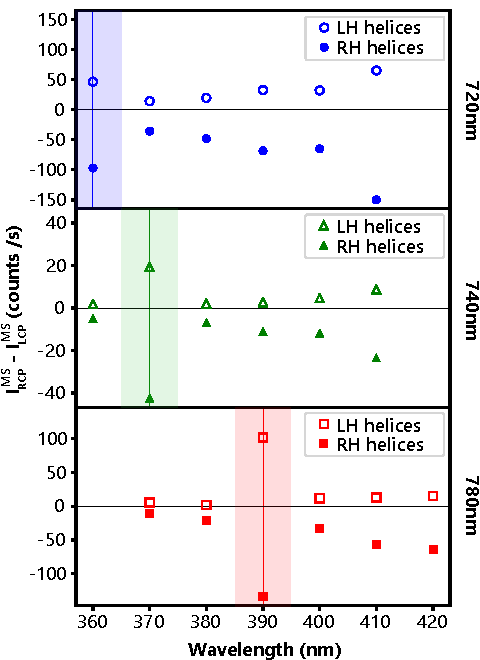
\includegraphics[scale=1]{./figures/results/HRS/hrs_cd_data.pdf}
    \caption{\label{fig:results:HRS:hrs_cd_data}
    Circular difference ($I_{RCP}^{MS}-I_{LCP}^{MS}$) in multiphoton scattering intensity, for both left-handed (LH) and right-handed (RH) nanohelix suspensions. Again, pump wavelengths of $\SI{720}{\nano\m}$, $\SI{740}{\nano\m}$ and $\SI{780}{\nano\m}$ are shown in blue, green, and red, respectively, and vertical coloured lines mark the HRS (second-harmonic) wavelength. The HRS circular difference clearly reverses between nanohelix enantiomorphs.}	
\end{figure}

Figure~\ref{fig:results:HRS:hrs_data} shows the obtained multiphoton scattering spectra for both left- and right-handed nanohelix suspensions, under LCP and RCP illumination at three fundamental wavelengths: $\SI{720}{\nano\m}$, $\SI{740}{\nano\m}$ and $\SI{780}{\nano\m}$ (shown in blue, green, and red respectively). 
The second-harmonic is marked by a vertical line, with the shaded region denoting the bandwidth of the band-pass filter used. At all three fundamental wavelengths, a clear peak is observed at the second-harmonic, corresponding to hyper-Rayleigh scattering well above the multiphoton luminescence background. Additionally, background measurements were taken by measuring the HRS of the sodium-citrate water solution, without nanohelices. In these experiments, no HRS \textit{or} multi-photon luminescence counts were detected during the 30 second counting window.

Importantly, a clear difference in HRS intensity between RCP and LCP illumination is also observed. 
This effect is emphasised in figure~\ref{fig:results:HRS:hrs_cd_data}, which shows the circular difference in multiphoton scattering intensities ($I_{RCP}^{MS}-I_{LCP}^{MS}$) for both enantiomorphs. At all three fundamental wavelengths, a clear peak in circular difference is observed at the second-harmonic, reversing sign between enantiomorphs indicating an intrinsically chiral origin. The HRS-CID is significantly larger than the neighbouring two- and three-photon luminescence CID, which are also recorded. 

\begin{figure}[htb!]	
    \centering	
    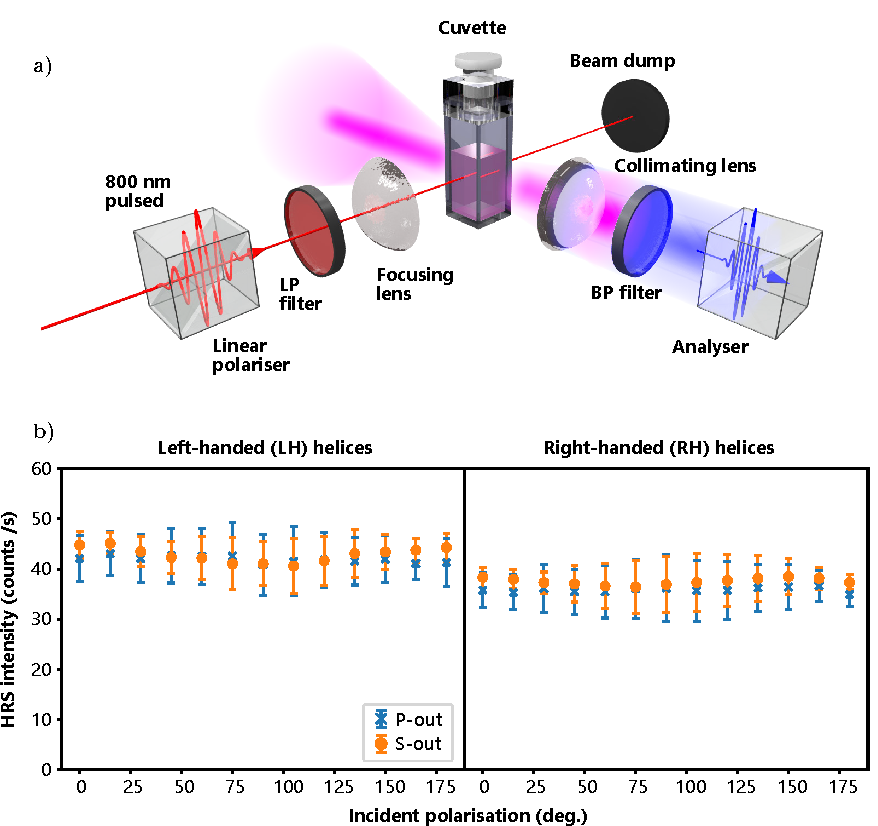
\includegraphics[scale=1]{./figures/results/HRS/hrs_linpol_data.pdf}
    \caption{\label{fig:results:HRS:hrs_linpol_data}
    The nanohelices are isotropically suspended in water. \textbf{a)} Schematic of the setup used to measure hyper-Rayleigh scattering of linearly polarised incident light. \textbf{b)} P-polarised (blue crosses) and S-polarised (orange dots) HRS intensity at $\SI{360}{\nano\m}$, as the polarisation of $\SI{720}{\nano\m}$ incident light is rotated. Both left-handed (LH) and right-handed (RH) nanohelix suspensions exhibit no variation outside of experimental uncertainty, demonstrating a clear isotropic arrangement of helices within the liquid suspension.}	
\end{figure}

To further verify the chiral origin of the measured HRS-CID, linearly polarised HRS measurements are performed. Figure~\ref{fig:results:HRS:hrs_linpol_data}a shows the setup used in these measurements. Here, the incident polarisation is linear and can be freely rotated. An analysing polariser is placed before the detector, allowing the HRS signal to be decomposed into P-polarised (horizontal) and S-polarised (vertical) components. Both left- and right-handed nanohelix suspensions were examined, at an incident wavelength of $\SI{720}{\nano\m}$, with a $\SI{360}{\nano\m}$ band-pass filter at the output, selecting the HRS. 
Figure~\ref{fig:results:HRS:hrs_linpol_data}b shows the P- and S-polarised components of HRS intensity as the incident polarisation is rotated. For both P- and S-polarised HRS, and for both enantiomorphs, it can be seen that HRS intensity remains constant. This result establishes an isotropic arrangement of nanohelices, and indicates a dipolar origin of the HRS response~\cite{Hao2002b, verbiest2009second}. 

Additional reference data was taken, but found to serve only as an interesting contrast to the anisotropy of the nanohelices. In order to measure an HRS reference for a fully isotropic medium, a water suspension of $\SI{20}{\nano\m}$ spherical Ag nanoparticles was studied using a similar method as in figure~\ref{fig:results:HRS:hrs_linpol_data}. Here however, the incident polarisation was fixed at either P- or S-polarised, and the analysing polariser freely rotated. 
It is important to also note that the spherical nanoparticle suspension is higher concentration ($116$ picomolar) than our nanohelix suspensions ($\approx 20$ picomolar), and the scattering cross section can vary significantly with shape.
Therefore, the following results should not be directly compared to those obtained for nanohelices.
The HRS intensity in this configuration is shown in figure~\ref{fig:results:HRS:hrs_spheres}. 
For P-polarised incident light, the analyser sweep shows a sinesoidal intensity curve, clearly showing a linearly polarised output. However, under S-polarised illumination, the measured signal reduces to near zero. This is because the nanospheres scatter in a dipole pattern originating from surface charge oscillations along the polarisation axis of incident light. 
In our experimental configuration, no dipole emission will propagate in the direction of the detector under S-polarised illumination. Conversely, P-polarised illumination will drive dipolar scattering with a P-polarised component in the direction of the detector. This data verifies one important aspect of the nanohelix samples: The helical geometry provides intrinsic chirality, however the helical axis acts, to some extent, as a rod. In this case, the nanohelices scatter in a dipole pattern originating from surface charge oscillations \textit{along the helical axis}, with an amplitude related to the angle between the helical axis, and the angle of incident polarisation. 
This results in a depolarisation effect, in which light is scattered equally at all polarisation angles due to the random orientation of the nanohelices, as observed in figure~\ref{fig:results:HRS:hrs_linpol_data}b.

\begin{figure}[htb!]	
    \centering	
    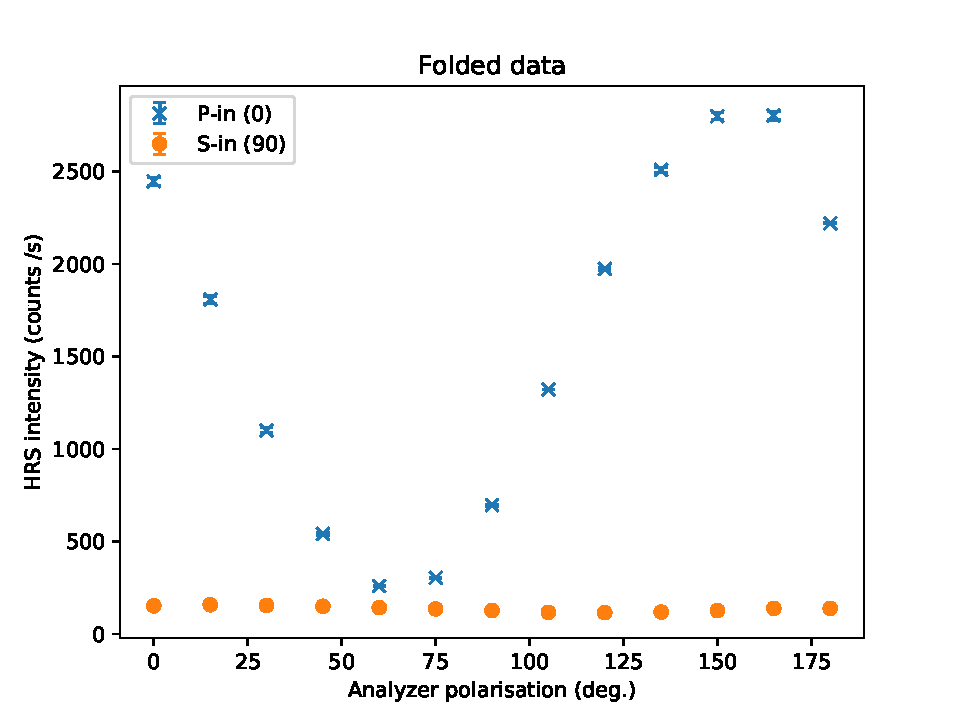
\includegraphics[scale=1.0]{./figures/results/HRS/hrs_spheres.pdf}
    \caption{\label{fig:results:HRS:hrs_spheres}
    HRS intensity from Ag nanospheres at $\SI{360}{\nano\m}$, under P-polarised (blue crosses) and S-polarised (orange dots) $\SI{720}{\nano\m}$ illumination, as the analysing polariser is rotated. P-polarised illumination results in linearly polarised emission, whereas S-polarised illumination results in almost zero intensity, both consistent with dipolar emission originating from charge oscillations in the direction of incident polarisation.}	
\end{figure}

\section{Discussion}

Within the electric dipole approximation, the second-order induced polarisation of a single scatterer is described by the hyper-polarisability tensor $\beta_{ijk}$. This tensor is similar in nature to the second-order susceptibility tensor discussed in section~\ref{sec:background:NonlinearOptics:susceptibility}, and relates the induced polarisation of the particle $\mu_{i}$ to a driving electric field by $\mu_{i}(2\omega) =  \epsilon_{0} \beta_{ijk} E_{j}(\omega) E_{k}(\omega)$. For a single scatterer, the HRS intensity is thus proportional to the square of the hyper-polarisability tensor $\beta_{ijk}^2$. In liquid suspensions, the total measured HRS intensity originates from the incoherent sum of randomly oriented scatterers within the illumination volume.
The measured HRS intensity is thus proportional to the rotational average of the square of the hyper-polarisability tensor $\langle I(2\omega) \rangle \propto \langle \beta^{2} \rangle$.
In a homogeneous suspension of structurally isotropic particles, HRS is forbidden within this electric dipole approximation. By acting on the hyperpolarizability tensor with rotation matrices for all 3 axes and equating to the unrotated tensor for any arbitrary rotation (thus enforcing true 3D isotropy), every component of the hyperpolarizability tensor reduces to zero.

In these experiments however, the individual nanostructures are anisotropic, but randomly oriented on average. During a single laser pulse, and over the sample volume, there will exist slight deviations from perfect average isotropy, an ``anisotropic excess''. The anisotropic excess prevents HRS from completely cancelling out, allowing for non-zero signal during that pulse, with intensity and polarisation dependent on the orientation of the anisotropic excess. By integrating over many pulses (our 30 second counting window), the orientational dependence of the HRS is averaged out, and general structural information can be obtained.
Mathematically, the averaging process is equivalent to integrating the HRS intensity from a single structure over all orientations, and can be described in terms of the normalised triple integral:
\begin{equation}
    \langle I(2\omega) \rangle \propto
    \left(\frac{1}{2\pi}\right)^3
    \int_{0}^{2\pi} \int_{0}^{2\pi} \int_{0}^{2\pi}
    \beta_{ijk} ^{\prime 2} (\theta, \phi, \psi)
    d\theta d\phi d\psi
\end{equation}
Note that this is different to symmetrising the tensor, which involves integrating $\beta$, rather than $\beta^{2}$. Similar to chapter~\ref{sec:results:OAinPlanarNanohelices}, $\beta_{ijk}^{\prime} (\theta, \phi, \psi)$ describes an effective hyper-polarisability tensor after rotation about the $z$, $y$, and $x$ axis by angles $\theta$, $\phi$, and $\psi$ respectively. In full tensor notation this is described in terms of the rotation matrices by (given in section~\ref{sec:background:NonlinearOptics:rotation}) by
\begin{equation}
    \begin{split}
        \beta_{ijk}^{(2) \prime} (\theta, \phi, \psi) =
        & R^{x}(\psi)_{i\alpha}R^{x}(\psi)_{j\beta}R^{x}(\psi)_{k\gamma} \\
        & R^{y}(\phi)_{i\alpha}R^{y}(\phi)_{j\beta}R^{y}(\phi)_{k\gamma} \\
        & R^{z}(\theta)_{i\alpha}R^{z}(\theta)_{j\beta}R^{z}(\theta)_{k\gamma}
        \beta_{\alpha \beta \gamma}^{(2)}
    \end{split}
\end{equation}
Applying parity inversion to the hyper-polarisability tensor using a reflection matrix $A_{ij}$, and performing the same averaging operation, produces an identical non-zero expression. While non-zero HRS is permitted, HRS-CID is forbidden within the electric dipole approximation. Surprisingly, clear HRS-CID was nevertheless experimentally observed. This strongly suggests that our nanohelix structures should not simply be treated as point-like scatterers described by hyper-polarisability tensors. Previous work has outlines two models for the nonlinear optical activity of chiral molecules, in terms of dominant magnetic dipole contributions, and dominant chirally-coupled electric dipole contributions~\cite{Fischer2005a}. By considering our nanohelix structures in the context of these molecular models, two potential origins of the observed HRS-CID are proposed.

The first potential origin is if the nanohelices does not behave as a point scatterers.
The nanohelix wire thickness is comparable to the materials skin depth, however the helix dimensions overall are significantly larger than this. Therefore, an individual helix can be modelled as a helical arrangement of oscillating achiral point-dipoles. These oscillating dipoles will be chirally coupled, and phase-retardation effects across the span of the helix, due to the chiral arrangement, can lead to a measurable HRS-CD.
Importantly, this description can be considered in terms of the nonlinear extension to Kuhn's coupled oscillator model of molecular chirality~\cite{Fischer2005a}.
The second potential origin is from higher-order contributions to HRS than electric dipoles. We have established that the signal is not of electric quadrupolar origin, from the results presented in figure~\ref{fig:results:HRS:hrs_linpol_data}b. However, magnetic-dipole contributions can not be ruled out by these results. 
In chapter~\ref{sec:results:OAinPlanarNanohelices} we disregarded the magnetic dipole contribution to nonlinear emission as negligible, primarily due to the orientation of helices relative to the incident light. In this experimental configuration however, this is not the case.
The helical structure acts as a conductive coil. Driving current along the length of the helix will induce a magnetic field parallel to the induced electric dipole. Now, the magnetic-dipole electric-dipole contribution to nonlinear emission cannot be considered negligible, and this contribution permits HRS-CID. The overall HRS signal would, in this case, be described by an electric dipole contribution exhibiting no CID, and a magnetic-dipole contribution from which the CID originates.
Interestingly, this description can be considered in terms of the nonlinear extension to the one-electron on a helix model of molecular chirality~\cite{Fischer2005a}.
While outside of the scope of this work, it may be possible to distinguish between the two models by measuring optical rotation effects in second-harmonic scattering, as optical rotation is permitted only in the chirally-coupled dipole description of nonlinear emission~\cite{Fischer2005a}.

For the purposes of comparison to the linear CD spectra, we can characterise the HRS-CD by a polarisation ellipticity:
\begin{equation}
    \theta^{HRS} (\text{deg.}) = \frac{180}{\pi} \tan\left( \frac{\sqrt{I_{RCP}^{HRS}} - \sqrt{I_{LCP}^{HRS}}}{\sqrt{I_{RCP}^{HRS}} + \sqrt{I_{LCP}^{HRS}}} \right).
\end{equation}
Here, $I_{RCP}^{HRS}$ and $I_{LCP}^{HRS}$ are the electric field intensities of light scattered at the second harmonic for RCP and LCP illumination, respectively. 
The measured linear and HRS ellipticities are given in table~\ref{table:HRS:ellipticity}. Note that in these data the linear- and HRS-CD are expected to have an opposite sign, due to experimental geometry.
Table~\ref{table:HRS:ellipticity} indicates that the measured HRS-CD effect is 3 to 4 times stronger than the linear CD across the range of wavelengths studied. However, when considering the volume of the liquid interacting with incident light, the HRS-CD effect appears significantly more sensitive than its linear counterpart. 
For a Gaussian beam, at a position $z$ from the focus, with a beam waist $w_0$ and a Rayleigh range $z(r)$, the beam radius $w(z)$ is given by $w(z) = {w_0}\sqrt {1 + (z/z_R)^2}$. 
We define the beam volume as the integral of the spot area $\pi w(z)^2$ between two positions $z_i$ (initial) and $z_f$ (final) as:
\begin{equation}
    V_{beam} = \int^{z_f}_{z_i} \pi \left( {w_0}^2 \sqrt {1 + (z/z_R)^2} \right)^2 dz.
\end{equation} 
For these experiments, we assume that significant HRS occurs within the Rayleigh range of the fundamental beam, and so the effective interaction volume is given by $V_{beam}$ integrated between $-z_R$ and $z_R$. 
Considering the $\SI{10}{\centi\m}$ focal length lens used in our experiments, with an incident beam of waist $\SI{1.2}{\milli\m}$ and $\lambda = \SI{740}{\nano\m}$ fundamental light, the waist at the focus ${w_f} = (\lambda f)/(\pi {w_0})$ is found to be $\approx \SI{20}{\micro\m}$, with a Rayleigh range of $\approx \SI{2}{\milli\m}$. From this, we assume that we measure HRS from a $\SI{4}{\milli\m}$ path length through the cuvette. 
The effective beam volume ($V_{beam}$) is then $\approx 10^{-11}\SI{}{\m\cubed}$ ($=\SI{10}{\nano\litre}$). 
By comparison, the commercial CD spectrometer uses a $\SI{10}{\milli\m}$ optical path length with an approximately constant beam radius of $\approx \SI{1}{\milli\m}$, giving an effective beam volume of  $\approx 10^{-6}\SI{}{\m\cubed}$ ($=\SI{1}{\milli\litre}$). 
This value is 5 orders of magnitude larger compared to the nonlinear case. Consequently, the HRS-CD effect is significantly more sensitive than its linear counterpart. 

\begin{table}[tbp]
    \begin{tabular}{llll}
    \firsthline
                                                                & \textbf{\begin{tabular}[c]{@{}l@{}}Fundamental \\ wavelength (nm)\end{tabular}} & \textbf{\begin{tabular}[c]{@{}l@{}}Linear \\ ellipticity (mdeg.)\end{tabular}} & \textbf{\begin{tabular}[c]{@{}l@{}}HRS \\ ellipticity (mdeg.)\end{tabular}} \\ 
    \hline
    \multirow{3}{*}{\begin{tabular}[c]{@{}l@{}}Right-handed \\ helices\end{tabular}}  & 720                                                                    & 920                                                                   & -3299                                                              \\
                                                                & 740                                                                    & 803                                                                   & -3356                                                              \\
                                                                & 780                                                                    & 569                                                                   & -1890                                                              \\ 
    \hline
    \multirow{3}{*}{\begin{tabular}[c]{@{}l@{}}Left-handed \\ helices\end{tabular}}& 720                                                                    & -370                                                                  & 1811                                                               \\
                                                                & 740                                                                    & -293                                                                  & 1455                                                               \\
                                                                & 780                                                                    & -164                                                                  & 1334                                                               \\ 
    \lasthline
    \end{tabular}
    \caption{Linear and HRS ellipticities for left- and right-handed nanohelix suspensions. Values are given at the three fundamental wavelengths used in the HRS experiments.}
    \label{table:HRS:ellipticity}
\end{table}


\section{Conclusions}
We have demonstrated the first observation of HRS-CD, by measuring multiphoton scattering spectra from a low concentration isotropic suspension of Ag nanohelices in water. Although complete macroscopic isotropy would forbid HRS, over the time scale of ultrashort laser pulses, and the low interaction volume used, deviations from perfect isotropy allow the chirality of the helices to be probed. In this sense, low concentrations of nanoparticles may in fact be an advantage. Low particle concentrations, and small interaction volumes, are more statistically likely to deviate from perfect isotropy, and over long counting windows, these deviations sum to give a measurable probe of intrinsic chirality.

This technique therefore allows pure chiral symmetry information to be obtained from extremely low concentrations of nanostructures suspended in low volumes of liquid. The range of available miniaturised cuvettes, narrow capillaries, microfluidic channels and hollow-core optical fibres position this new chiroptical characterisation directly within the lab-on-a-chip paradigm. Additionally, since plasmonic nanoparticles can be leveraged to increase the chiroptical response of molecules, this technology potentially allows the miniaturised characterisation of synthesised chemicals. 

